\documentclass[tikz,border=5pt]{standalone}
\usepackage{amssymb,amsmath}
\usepackage{tikz}
\usepackage{lmodern}
\usetikzlibrary{calc}

\begin{document}
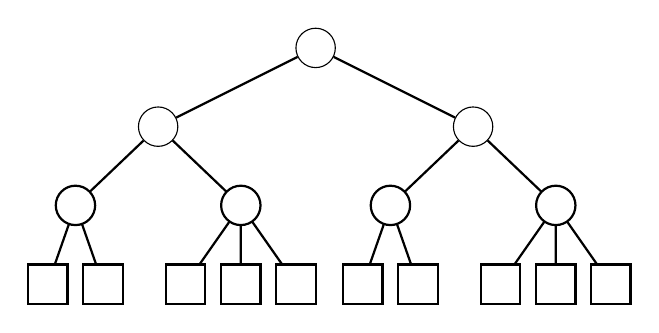
\begin{tikzpicture}[
	edge from parent/.style={draw, thick},
	every node/.style={draw, minimum size=5mm, inner sep=0pt},
	circ/.style={circle},
	sq/.style={rectangle},
	level distance=10mm,
	level 1/.style={sibling distance=40mm},
	level 2/.style={sibling distance=21mm},
	level 3/.style={sibling distance=7mm}
	]
	\node[circ] {}
	child { node[circ] {}
		child { node[circ] {}
			child { node[sq] {} }
			child { node[sq] {} }
		}
		child { node[circ] {}
			child { node[sq] {} }
			child { node[sq] {} }
			child { node[sq] {} }
		}
	}
	child { node[circ] {}
		child { node[circ] {}
			child { node[sq] {} }
			child { node[sq] {} }
		}
		child { node[circ] {}
			child { node[sq] {} }
			child { node[sq] {} }
			child { node[sq] {} }
		}
	};
\end{tikzpicture}

\end{document}